\documentclass[5pt]{article}
\usepackage{multicol,multirow}
\usepackage{graphicx} % Required for inserting images
\usepackage[margin=0.75cm]{geometry}
\usepackage{xcolor}
\usepackage{amsmath,esint}
\usepackage{mathtools}
\usepackage{relsize}
\usepackage{mathtools}
\usepackage{nccmath}
\usepackage[inline]{enumitem}
\usepackage{algpseudocode}

\usepackage{empheq}
\usepackage{amsfonts}

\usepackage{tkz-euclide}
\usepackage{tikz}

\definecolor{LightGray}{gray}{0.9}

\usepackage{minted}

\newenvironment{amatrix}[1]{%
  \left[\begin{array}{@{}*{#1}{c}|c@{}}
}{%
  \end{array}\right]
}

\DeclarePairedDelimiter\abs{\lvert}{\rvert}%
\DeclarePairedDelimiter\norm{\lVert}{\rVert}%
\newcommand{\universalSet}{\mathbb{U}}

\makeatletter
\let\oldabs\abs
\def\abs{\@ifstar{\oldabs}{\oldabs*}}

\newcommand{\tr}[3]{
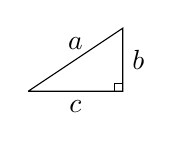
\begin{tikzpicture}[scale=0.40]
    \coordinate [] (A) at (-1.5cm,-1.cm);
    \coordinate [] (C) at (1.5cm,-1.0cm);
    \coordinate [] (B) at (1.5cm,1.0cm);
    \draw (A) -- node[above] {$a$} (B) -- node[right] {$b$} (C) -- node[below] {$c$} (A);
    \draw (1.25cm,-1.0cm) rectangle (1.5cm,-0.75cm);
\end{tikzpicture}
}


\begin{document}

\newtheorem{theorem}{Theorem}
\newtheorem{lemma}{Lemma}
\newtheorem{properties}{Properties}
\newtheorem{axiom}{Axiom}


\begin{center}
     \Large{\textbf{Discrete Mathematics}}\\
     \small{Class: MATH 2410}\hfill\small{\textcopyright Maximilien Notz \the\year{}}
     \noindent\rule{20.2cm}{0.4pt}
\end{center}

\begin{multicols}{2}
\setcounter{secnumdepth}{0}

\subsection{Standard Binary Encodings}
\subsubsection{Integers}
\textbf{Sign bit:} The first bit is used to indicate the sign of the number, with 0 representing positive and 1 representing negative.\\
\textbf{Two's complement:} Negation is done by inverting all bits and adding 1.\\
\textbf{Offset binary:} Labeling the values of a binary number system from the minimum value to the maximum value, with the midpoint being zero. For example, in an 8-bit offset binary system, the values range from -128 to 127, with 0 represented as 10000000.\\


\subsubsection{Real Numbers}
Suppose 32 bits are used to represent a real number.
The first bit is the sign bit, the next 8 bits are the exponent, and the last 23 bits are the mantissa. 
The exponent is stored in \textbf{offset binary} notation. The mantissa is stored in normalized form, meaning that the leading 1 is not stored.

\end{multicols}
\subsection{General Tips}
\begin{itemize*}
    \item $\sqrt{x^2}=|x|,x\in\mathbb{R}$
    \item $(\sqrt{x})^2=x, x\geq 0$
    \item $\sum_{i=1}^{n}i=\frac{n(n+1)}{2}$
    \item $\sum_{i=1}^{n}i^2=\frac{n(n+1)(2n+1)}{6}$\\
    \item $(a+b)^3=a^3+b^3+3ab(a+b)$
    \item $(a-b)^3=a^3-b^3-3ab(a-b)$
    \item $a^3+b^3=(a+b)(a^2-ab+b^2)$
    \item $a^3-b^3=(a-b)(a^2+ab+b^2)$
\end{itemize*}
\end{document}
